\section{Evaluation}
\subsection{Process}
Evaluating the process of designing and building a system.

\subsubsection{Design/Pre-Development} 

Software design and the ratio of time spent on design over development is a debated topic within the industry, the most popular theory currently being \textit{Agile} which is biased towards development over design whereas \textit{Waterfall} considered a legacy methodology believes in designing the entire solution before development can take place.

I focused my design on gaining knowledge of the technologies I had no previous experience: \keyword{blockchain} interaction and \keyword{smart contract} design. Only abstract models of the system were drawn so I could research all the needed technology.

% maybe some pictures of my early diagrams, in notebook.

In practice this strategy was reasonably successful as the overall architecture is representative of my original design, in spite of this many key systems were underestimated or poorly designed largely thanks to lack of knowledge. Although this is how agile development is supposed to work, it's okay if fundamental change happens in fact you should always consider change and change quickly.

\subsubsection{Development}

As far as timing development was perfect, every deadline was hit on time with no need for extension or reevaluation. I put this down to aggressive and continuous scope handling, it's very easy as an engineer to completely over-engineer a system and I've had problems managing this desire in the past. However for this project I clearly defined the scope in my mind so whenever new complexity was being debated I always forced myself to consider scope and time constraints.

As a result if you read all my \href{https://github.com/MrHarrisonBarker/CRPL/blob/main/README.md}{sprint reviews} and burndown graphs I consistently hit deadlines and manage the amount of work assigned to each sprint. 

In conjunction with agile development I also initially planned to use a development workflow called \textbf{TDD} (\textbf{T}est \textbf{D}riven \textbf{D}evelopment) that says functionality should first be test cases the developer then aims to pass by implementing functionality. It's very popular in the \textit{Agile} space and can increase code quality and speed up development, however functionally limited when used in larger user focused and very infrastructure heavy systems. I still tested heavily but my implementation wasn't dependent on testing.

\begin{figure}[H]
\caption{example burndown for sprint 2}
\centering
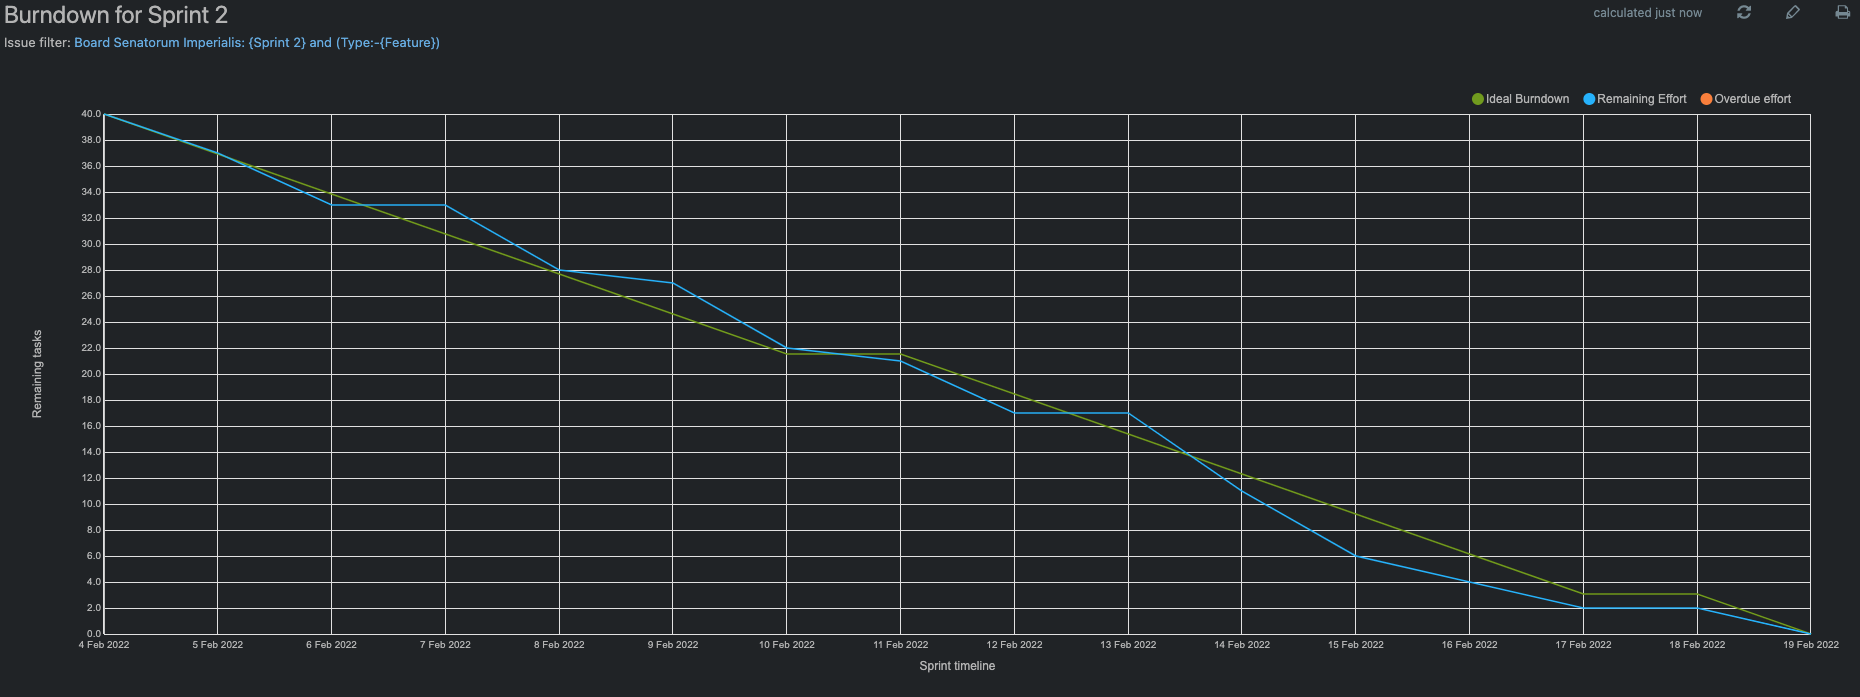
\includegraphics[width=\textwidth,height=\textheight,keepaspectratio]{images/burndown-2}
\end{figure}

\subsubsection{Was it agile?}

To assess if my process has been agile I'll being using the 4 values from the agile manifesto\cite{agile}

\begin{description}
	\item[Individuals and interactions over processes and tools] isn't very applicable as this is an individual project.
	\item[Working software over comprehensive documentation] links back to my troubles with \textbf{TDD} I was focusing more on passing the test than what the software need to do. 
	\item[Customer collaboration over contract negotiation] is an area I could've done a lot more in, my customer is an imagined aggregate of certain struggles not a real person this could've been a better representation with more hands on research.
	\item[Responding to change over following a plan] would be a great summary of this project because although I had a fairly comprehensive plan I only every took it as a guide, If I'd spent weeks on a master plan it would've only been a waste of time.
\end{description}

\subsection{Product}
Evaluating the system that has been built functionally and non-functionally.

\subsubsection{Functional specification}

Have I built a system that satisfies my specification?

\begin{figure}[H]
\caption{success of each functional requirement}
\begin{table}[H]
\begin{tabular}{|p{0.2\textwidth}|p{0.8\textwidth}|}
\hline
Feature                         & Successfully implemented?                                                                                                                                                                                                                                                                                                                                                           \\ \hline
Copyright smart contract        & A fully featured copyright contract has been built and deployed onto a test blockchain, the contract is capable of registering a copyrighted work with sufficient metadata to establish ownership and specific legal protections.                                                                                                                                                   \\ \hline
Multi-party distribution        & Ownership of a registered work is represented as a multi-party share structure allowing many authors to have "ownership" of a single work.                                                                                                                                                                                                                                          \\ \hline
Ownership transfer              & The ownership of a registered work can be changed via a proposal and vote system requiring the unanimous consensus of all current owners. *Voting is not majority share-based like limited companies.                                                                                                                                                                               \\ \hline
Work verification               & Verification of works is currently simple using hash comparison, this finds complete file accurate copies and so therefore even simply adding a zero or null data to the file bypasses verification. To solve this problem more complex algorithms will be needed or the use of third-party services, this was outside the scope of this project.                                   \\ \hline
Dispute filing                  & The system allows anyone (except the owner) to dispute a registered work for a given reason and the choice of an expected recourse (ownership change or payment). Right owners can then either reject the dispute or accept and apply the expected recourse.                                                                                                                        \\ \hline
Digital signing                 & Once a work has been registered we inject metadata into the uploaded file for proof of registration, this is done two ways: custom singers built for supported file types and a universal signer that inserts data at the end of any file type.                                                                                                                                     \\ \hline
Decentralised Work CDN \& proxy & All registered works are automatically saved to IPFS (InterPlanetary File System) which is a peer to peer network for storing files distributed securely in chunks over multiple nodes. A user can then access this file either through an official gateway (ipfs.io/ipfs/), running your own node to connect to the network or my public gateway (ipfs.harrisonbarker.co.uk/ipfs). \\ \hline
Websocket updates               & All updates are done through a single WebSocket, users are subscribed to works and applications when they click on them or have ownership associated with them.  The implementation of this is crude though as it was an extra feature added minimally towards the end of the development cycle with many concerns of scaling issues.                                               \\ \hline

\end{tabular}
\end{table}
\end{figure}

\subsubsection{Is it fit for purpose}

Have I built a system that addresses my issues with \keyword{copyright} discussed in \autoref{sec:unfit}? My stated three factors were \textit{complexity, jurisdiction dependence and lack of digital computerised systems}, does my system solve any of these?

First is complexity, by removing as much legal jargon from the process and a customisable protections system users know exactly how their work is protected without the need for legal council or manager therefore empowering creators. 

Next is jurisdiction dependence which is an escapable fact of the legal and governmental world that can cause issue and confusion when faced with a global internet culture. My system is global both because of \keyword{Ethereum} and its independence from any government.

Lastly digitalisation/computerisation, my system is computerisation of \keyword{copyright} law which solves my last two points but more importantly it's built for copyrightable digital work which traditional \keyword{copyright} is lacking in. Standardised digital signing and verification is proof of this ambition.

\subsubsection{Testing}

The system has been extensively unit tested at three levels: \keyword{smart contract}, back-end and front-end middleware.

Because contracts run within the \keyword{EVM} a testing environment is needed in this case \href{https://hardhat.org/}{Hardhat} which allows me to deploy and run tests on a \keyword{smart contract}.

\begin{figure}[H]
\caption{\href{https://github.com/MrHarrisonBarker/CRPL/blob/main/CRPL.Contracts/test/Copyright/Register.ts}{Register.ts} unit test snippet}
\centering
\begin{lstlisting}[language=JavaScript]
it('Should REVERT no shareholders', async function ()
{
	await expect(deployedContract.Register([], meta)).to.be.revertedWith('NO_SHAREHOLDERS');
});

it('Should REVERT when invalid shareholders', async function ()
{
	await expect(deployedContract.Register([{owner: ethers.constants.AddressZero, share: 1}], meta)).to.be.revertedWith('INVALID_ADDR');
});
\end{lstlisting}
\end{figure}

This is what the tests look like there're then run outputting statistics for each payable transaction on the contract including deployment. all \keyword{smart contract} test can be found \href{https://github.com/MrHarrisonBarker/CRPL/tree/main/CRPL.Contracts/test}{here}.

\begin{figure}[H]
\caption{contract statistics from Hardhat}
\centering
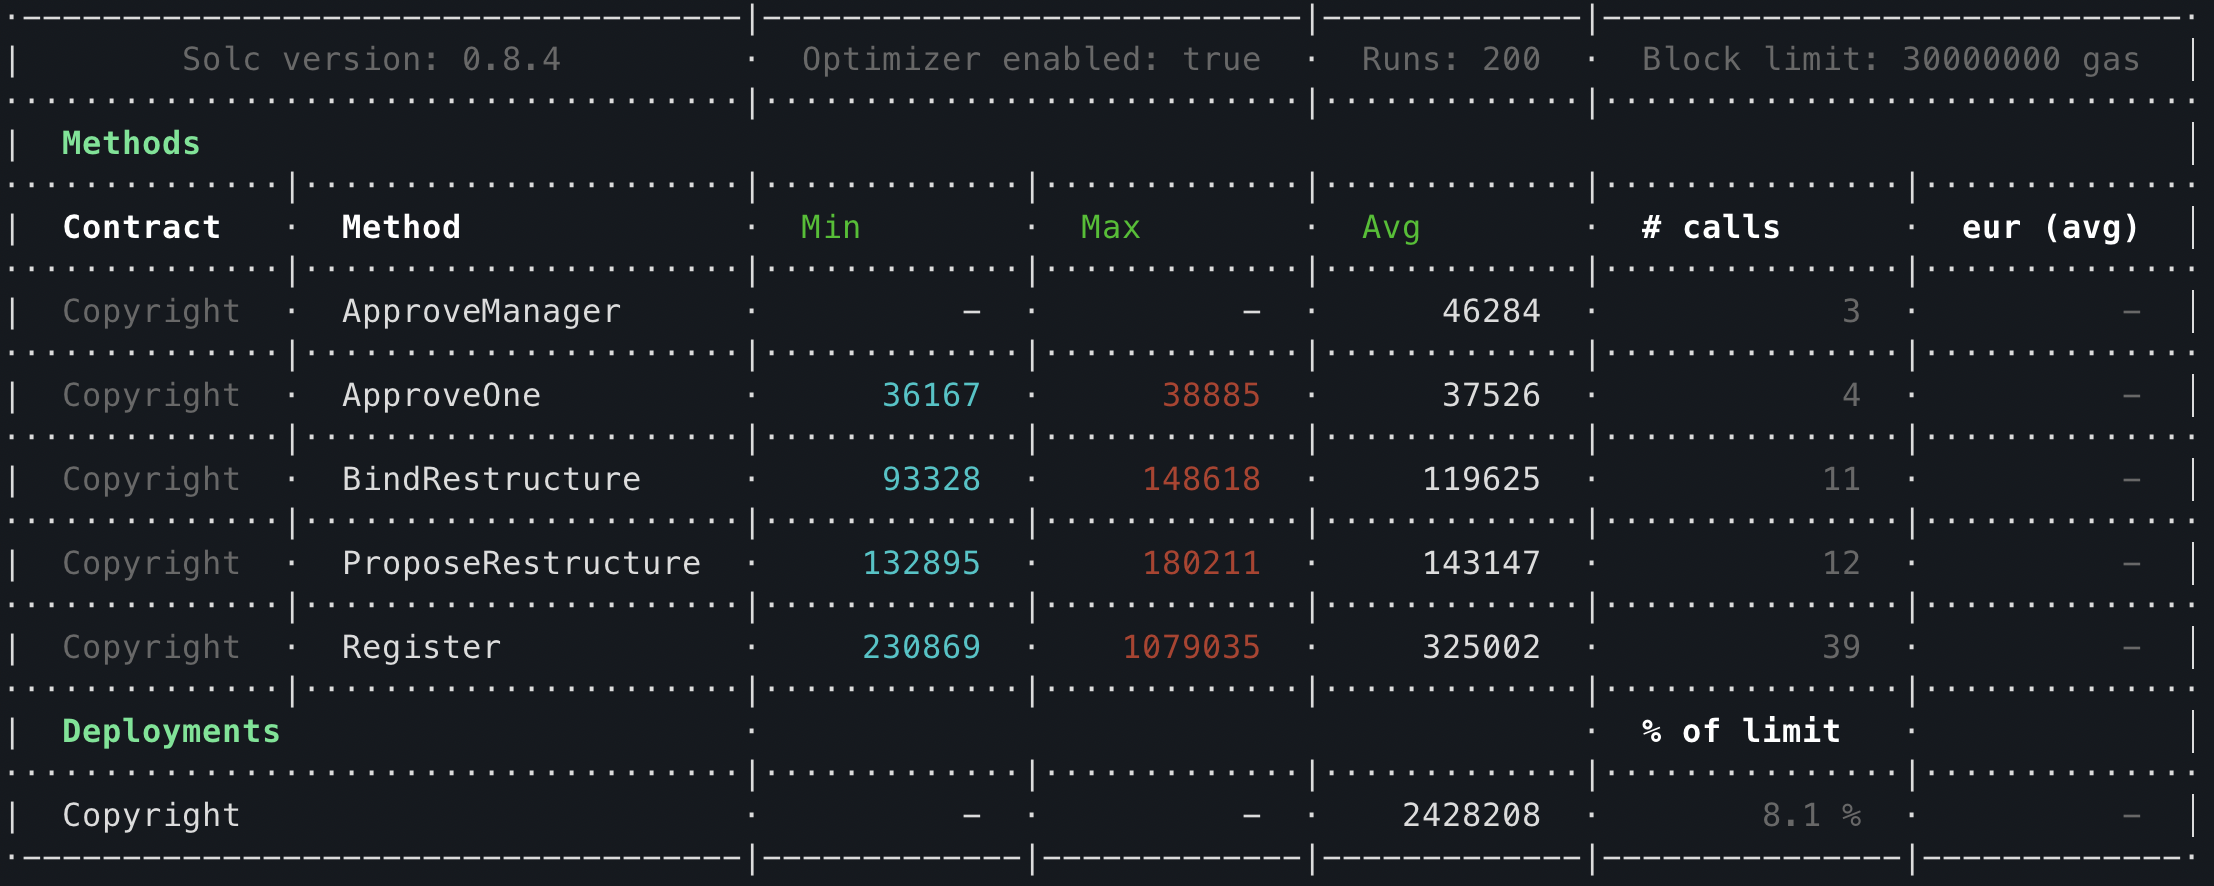
\includegraphics[width=\textwidth,height=0.4\textheight,keepaspectratio]{images/appendix/tests/hardhat-results}
\centering
\end{figure}

Back-end tests are written in the \href{https://github.com/MrHarrisonBarker/CRPL/tree/main/CRPL.Tests}{CRPL.Tests} project separated by domain all using \href{https://nunit.org/}{NUnit} test framework and runner.

\begin{figure}[H]
\caption{Back-end test directory structure}
\hfill
\subfigure{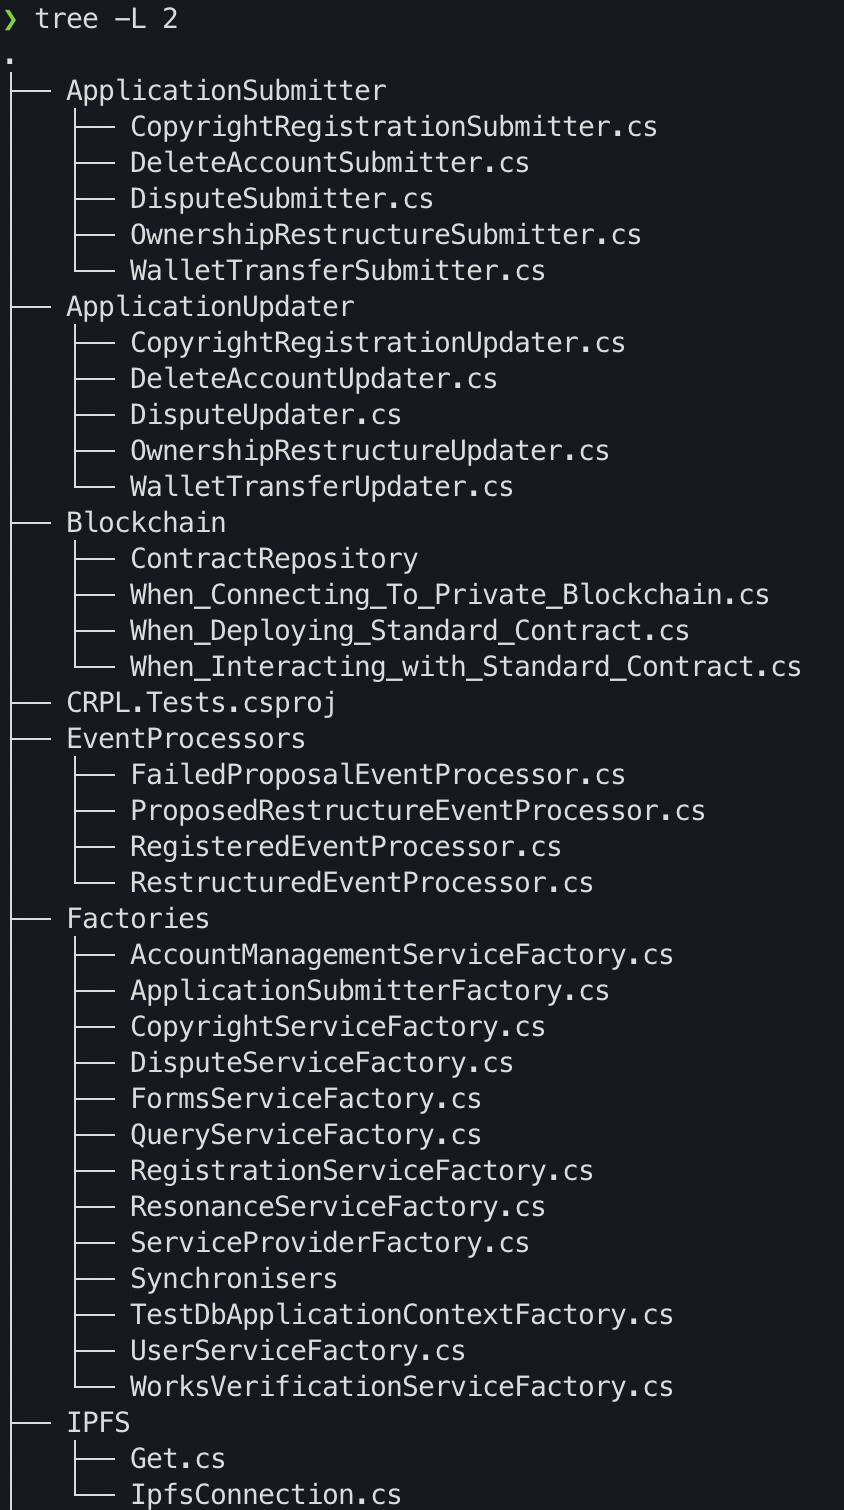
\includegraphics[width=\textwidth,height=0.5\textheight,keepaspectratio]{images/appendix/tests/test-tree-1}}
\hfill
\subfigure{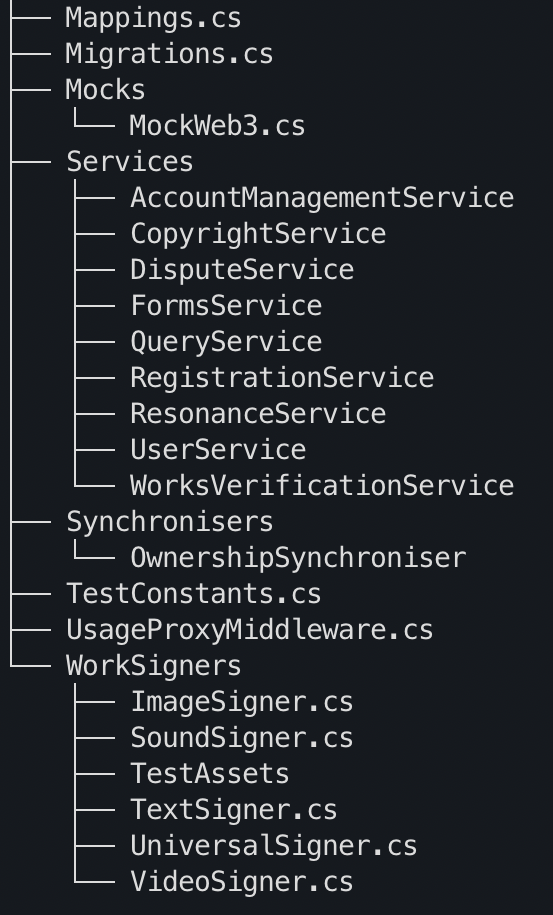
\includegraphics[width=\textwidth,height=0.3\textheight,keepaspectratio]{images/appendix/tests/test-tree-2}}
\hfill
\end{figure}

The front-end logic is tested using Angular's built in test framework \href{https://jasmine.github.io/}{Jasmine} found in \textit{.spec.ts} files.

\begin{figure}[H]
\caption{\href{https://github.com/MrHarrisonBarker/CRPL/blob/main/CRPL.Web/ClientApp/src/app/_Services/auth.service.spec.ts}{auth.service.spec.ts} nonce fetch test}
\centering
\begin{lstlisting}[language=JavaScript]
it('should fetch nonce', inject(
      [HttpTestingController, AuthService],
      (httpMock: HttpTestingController, authService: AuthService) =>
      {
        let mockNonce: string = "TEST NONCE";
        service['Address'] = 'TEST ADDRESS';

        authService.fetchNonce().subscribe((nonce: string) =>
        {
          expect(nonce).toEqual("TEST NONCE")
        });

        let request = httpMock.expectOne("user/nonce?walletAddress=TEST%20ADDRESS");

        expect(request.request.responseType).toEqual('json');
        expect(request.cancelled).toBeFalsy();

        request.flush(mockNonce);
      }
    )
  );
\end{lstlisting}
\end{figure}

\textbf{All test reuslts can be found in appendix \ref{sec:test-results}}


